% Provenance (never printed): see sources/outline_sources.md (Year 3:
% radial velocity, transits, imaging and microlensing; what has been
% found; atmospheres from transmission spectra).
% Brief: sources/book5/BRIEFS.md, ch. 28. Curves from figdata/bachelor-3/
% rv_transit.py (Keplerian radial-velocity curves, a limb-darkened transit
% light curve computed by numerical integration, point-lens microlensing)
% and exoplanet_archive.py (the NASA Exoplanet Archive's composite table of
% confirmed planets, fetched 2026-10-23, with the model mass--radius curves
% of Zeng et al.). Exercise and problem values in the Book 5 scratch
% calculator calc/ch28.py. Selene's Lamp and its planet are invented.
\chapter{Exoplanètes}\label{ch:b3:exoplanets}

À l'automne 1994, deux astronomes mesurant les vitesses de 142
étoiles constatent que l'une d'entre elles, 51~Pegasi, se rapprochait de nous et s'éloignait
de nous avec une période d'environ quatre jours. La demi-amplitude du mouvement était
\qty{59}{m.s^{-1}}, soit quatre fois ce que leur spectrographe pouvait détecter. Le
compagnon qui entraînait l'étoile dans son mouvement avait au moins la moitié de la masse de
Jupiter, sur une orbite de \qty{0.05}{au}, huit fois plus proche de son étoile
que Mercure ne l'est du Soleil. Aucune théorie de formation planétaire n'avait de place
pour un tel corps. La découverte, annoncée en octobre 1995, ouvrit un nouveau champ
de l'astronomie~: trois décennies plus tard, plus de six mille planètes autour
d'autres étoiles sont confirmées, quelques-unes ont été observées directement, et
l'atmosphère de certaines a été analysée. Ce chapitre montre comment repérer des planètes trop
faibles pour être vues, ce qui a été trouvé et comment on lit
leurs atmosphères.
% ledger: nobel19:51peg, planet:Mercury.dist, data:b5-pscomp

\begin{recall}
L'effet Doppler, la vitesse radiale, les binaires spectroscopiques, les lois de
Kepler, le problème à deux corps et son centre de masse, la loi de Planck et la
hauteur d'échelle d'une atmosphère isotherme figurent dans les volumes de physique. Une
exoplanète et la zone habitable d'une étoile figurent dans les manuels scolaires. Le
flux et la luminosité d'une source figurent dans le volume de première année, dans son
chapitre sur les télescopes et la photométrie~; la température d'équilibre, dans son
chapitre sur la planétologie comparée. La formation planétaire et la ligne des glaces
figurent dans le volume de deuxième année. L'\omterm{def:b3:planetary-atmospheres:jeans-escape}{échappement de Jeans} et l'\omterm{def:b3:planetary-atmospheres:hydrodynamic}{échappement
hydrodynamique} et les limites de la zone habitable figurent dans ce volume, dans son
chapitre sur les atmosphères planétaires.
\end{recall}

\section{La méthode des vitesses radiales}\label{sec:b3:exoplanets:rv}

Une planète ne gravite pas autour de son étoile~: les deux corps tournent autour de leur centre de masse commun.
L'étoile, bien plus lourde, décrit une petite orbite qui lui est propre, et sa lumière
est alternativement décalée vers le rouge et vers le bleu, avec la période de la planète.

\begin{definition}[Méthode des vitesses radiales~; masse minimale]\label{def:b3:exoplanets:rv}
La \emph{méthode des vitesses radiales}\index{méthode des vitesses radiales} détecte une
planète par la variation périodique de la vitesse radiale de son étoile,
mesurée à partir du décalage Doppler des raies du spectre de l'étoile. Lorsque
l'inclinaison $i$ de l'orbite par rapport au plan du ciel est inconnue, elle
ne mesure que le produit $m_p\sin i$ de la masse de la planète par le sinus de
l'inclinaison, soit la \emph{masse minimale}\index{masse minimale} de la
planète.
\end{definition}

\begin{theorem}[Demi-amplitude de la vitesse radiale]\label{thm:b3:exoplanets:semi-amplitude}
Une étoile de masse $M_\star$ et une planète de masse $m_p$ sur une orbite circulaire de
période $P$ et d'inclinaison $i$, donnent à l'étoile une vitesse radiale
$v_r(t) = \gamma + K\cos\bigl(2\pi(t - t_0)/P\bigr)$, avec $\gamma$ la
vitesse du centre de masse et la demi-amplitude
\[
K = \left(\frac{2\pi G}{P}\right)^{1/3}
    \frac{m_p\sin i}{(M_\star + m_p)^{2/3}} .
\]
Sur une orbite d'excentricité $e$, la courbe n'est plus une sinusoïde,
$v_r = \gamma + K\bigl[\cos(\nu + \omega) + e\cos\omega\bigr]$, avec $\nu$
l'anomalie vraie et $\omega$ l'argument du périastre, et $K$ est
divisé par $\sqrt{1 - e^2}$.
\end{theorem}

\begin{proof}
Pour l'orbite circulaire~: la séparation $a$ des deux corps obéit
à la troisième loi de Kepler, $a^3 = G(M_\star + m_p)P^2/4\pi^2$. L'étoile se trouve à
la distance $a_\star = a\,m_p/(M_\star + m_p)$ du centre de masse
et parcourt son cercle à la vitesse $v_\star = 2\pi a_\star/P$. D'où
\[
v_\star = \frac{2\pi}{P}\,\frac{m_p}{M_\star + m_p}
          \left(\frac{G(M_\star + m_p)P^2}{4\pi^2}\right)^{1/3}
        = \left(\frac{2\pi G}{P}\right)^{1/3}\frac{m_p}{(M_\star + m_p)^{2/3}} .
\]
La ligne de visée fait l'angle $\pi/2 - i$ avec le plan de
l'orbite, si bien que seule la composante $v_\star\sin i$ de la vitesse de l'étoile s'y trouve, et
cette composante tourne avec l'étoile~: $v_r - \gamma = v_\star\sin i\,
\cos\bigl(2\pi(t - t_0)/P\bigr)$. La forme excentrique découle de
l'ellipse keplérienne et est admise.
\end{proof}

Puisque la planète est beaucoup plus légère que son étoile, $K$ fixe $m_p\sin i$
dès que la période est mesurée et que la masse de l'étoile est connue par son
spectre. Pour 51~Pegasi~b, $K = \qty{59}{m.s^{-1}}$ et $P = \qty{4.23}{d}$
autour d'une étoile d'une masse solaire donnent $m_p\sin i = 0.47$ masses jupitériennes.
Jupiter fait varier la vitesse du Soleil de \qty{12.5}{m.s^{-1}} sur son
orbite de \num{4331}~jours~: un observateur lointain verrait la vitesse du Soleil
osciller d'environ \qty{\pm 13}{m.s^{-1}} sur douze ans. La Terre fait varier la vitesse du Soleil de
\qty{9}{cm.s^{-1}}. Le spectrographe qui a découvert 51~Pegasi~b atteignait
\qty{13}{m.s^{-1}}~; ses successeurs atteignent environ \qty{1}{m.s^{-1}} (soit
une allure de marche de \qty{3.5}{km/h}), et le plus récent est conçu pour environ
\qty{10}{cm.s^{-1}}, de quoi détecter une planète de masse terrestre dans la zone
habitable d'une étoile de faible masse, où l'orbite de la planète est courte et où l'étoile est peu massive.
L'étoile elle-même impose une limite inférieure~: les pulsations et les taches de sa surface,
entraînées par sa rotation, décalent elles aussi ses raies, et le signal d'une planète
doit pouvoir être séparé de ces effets.
% ledger: nobel19:51peg, nobel19:sun-jupiter, nobel19:migration, planet:Jupiter.mass, planet:Jupiter.Porb, planet:Jupiter.ecc, planet:Earth.mass, sun:mass, eso:espresso, const:G

\begin{omfigure}
\centering
\begin{tikzpicture}
\begin{axis}[width=0.86\linewidth, height=0.40\linewidth,
  xmin=0, xmax=2, ymin=-40, ymax=42,
  xlabel={phase orbitale (en périodes)}, ylabel={$v_r - \gamma$ (\unit{m.s^{-1}})},
  tick label style={font=\scriptsize}, label style={font=\small},
  legend style={font=\scriptsize, at={(0.5,-0.30)}, anchor=north, legend columns=2, draw=none, cells={anchor=west}, /tikz/every even column/.append style={column sep=1em}}]
\addplot[thin, black!40, forget plot] coordinates {(0,0) (2,0)};
\addplot[thick, omDef] table[x=phase, y=v_circ] {figdata/out/bachelor-3-rv_transit-rv.dat};
\addlegendentry{orbite circulaire}
\addplot[thick, dashed, red!70!black] table[x=phase, y=v_ecc] {figdata/out/bachelor-3-rv_transit-rv.dat};
\addlegendentry{$e = 0.3$, $\omega = \ang{60}$}
\draw[<->, thick] (axis cs:1.0,0) -- (axis cs:1.0,30);
\node[font=\scriptsize, anchor=east] at (axis cs:0.99,12) {$K$};
\end{axis}
\end{tikzpicture}
\par\smallskip{\small La vitesse radiale d'une étoile accompagnée d'une planète, sur
deux orbites, pour une planète fictive de $K = \qty{30}{m.s^{-1}}$ et une
période de dix jours. Sur une orbite circulaire (trait plein), la courbe est une sinusoïde
de demi-amplitude $K$. Sur une orbite excentrique (tirets), l'étoile se déplace
le plus vite au voisinage du périastre, et la courbe devient dissymétrique~: ses extrema valent
$K(1 \pm e\cos\omega)$ et l'amplitude crête à crête reste
$2K$.}\label{fig:b3:exoplanets:rv}
\end{omfigure}

\section{Transits}\label{sec:b3:exoplanets:transits}

Si l'orbite est vue presque de côté, la planète passe devant son étoile
une fois par orbite et masque une petite partie de son disque.

\begin{definition}[Méthode des transits~; profondeur de transit~; paramètre d'impact]\label{def:b3:exoplanets:transit}
La \emph{méthode des transits}\index{méthode des transits} détecte une planète par
l'affaiblissement périodique de son étoile lorsque la planète traverse le disque stellaire. La
\emph{profondeur de transit}\index{profondeur de transit} $\delta$ est la baisse relative
du flux de l'étoile pendant le transit. Le \emph{paramètre d'impact}\index{paramètre d'impact (transit)}
$b = a\cos i/R_\star$ est la plus petite distance entre les centres de la planète et
de l'étoile, vus sur le ciel, exprimée en rayons stellaires $R_\star$, pour
une orbite de rayon $a$ et
d'inclinaison $i$.
\end{definition}

\begin{proposition}[Profondeur de transit]\label{prop:b3:exoplanets:depth}
Une planète sombre de rayon $R_p$ entièrement devant une étoile
d'éclat uniforme donne la profondeur $\delta = (R_p/R_\star)^2$.
\end{proposition}

\begin{proof}
La planète masque l'aire $\pi R_p^2$ d'un disque d'aire $\pi R_\star^2$
qui est également brillant partout~; le flux baisse dans la même proportion.
\end{proof}

Jupiter devant le Soleil réduirait son éclat de \qty{1.06}{\percent}, la Terre
de \num{84} parties par million~: la première est à la portée d'un petit
télescope, la seconde demande un télescope spatial qui mesure des milliers d'étoiles
pendant des années. Le disque stellaire n'est pourtant pas uniforme.

\begin{definition}[Assombrissement centre-bord]\label{def:b3:exoplanets:limb}
L'\emph{assombrissement centre-bord}\index{assombrissement centre-bord} est la diminution de la luminosité de surface
d'une étoile, du centre de son disque à son bord, le «~limbe~».
Près du bord, la ligne de visée traverse obliquement l'atmosphère de l'étoile
et atteint la profondeur optique unité dans des couches plus hautes et plus froides, qui
émettent moins. On l'écrit souvent comme une loi quadratique en $\mu = \cos\theta =
\sqrt{1 - r^2}$, où $r$ désigne la distance au centre du disque, exprimée
en rayons stellaires~: $I(\mu)/I(1) = 1 - u_1(1 - \mu) - u_2(1 - \mu)^2$.
\end{definition}

Une planète proche du centre d'un disque à \omterm{def:b3:exoplanets:limb}{assombrissement centre-bord} masque une lumière plus vive
que la moyenne et creuse davantage le transit~; près du bord, elle masque moins. Le
fond de la courbe de lumière est arrondi, et ses bords s'adoucissent. La durée
d'un transit porte la géométrie.

\begin{theorem}[Durée du transit]\label{thm:b3:exoplanets:duration}
Pour une orbite circulaire de période $P$, de rayon $a$ et d'inclinaison $i$, avec
$p = R_p/R_\star$ et \omterm{def:b3:exoplanets:transit}{paramètre d'impact} $b$, le temps écoulé entre le premier
contact et le dernier vaut
\[
T_{14} = \frac{P}{\pi}\arcsin\!\left(\frac{R_\star}{a}\,
          \frac{\sqrt{(1 + p)^2 - b^2}}{\sin i}\right),
\]
et le temps entre le deuxième et le troisième contact, lorsque la planète est
entièrement à l'intérieur du disque, $T_{23}$, est donné par la même formule, avec
$1 - p$ à la place de $1 + p$.
\end{theorem}

\begin{proof}
Posons $\varphi = 2\pi t/P$ la phase orbitale comptée à partir du milieu du transit.
Projeté sur le ciel, avec $x$ le long de la trajectoire de la planète et $y$ perpendiculairement à celle-ci,
le centre de la planète se trouve en $x = a\sin\varphi$ et $y = a\cos i\cos\varphi$
par rapport au centre de l'étoile. En rayons stellaires, le carré de la séparation vaut
\[
z^2 = \left(\frac{a}{R_\star}\right)^2(\sin^2\varphi + \cos^2 i\cos^2\varphi)
    = \left(\frac{a}{R_\star}\right)^2\sin^2 i\,\sin^2\varphi + b^2 .
\]
Les disques se touchent de l'extérieur lorsque $z = 1 + p$, en
$\sin\varphi = \sqrt{(1 + p)^2 - b^2}\,R_\star/(a\sin i)$, symétriquement
par rapport au milieu du transit. Le transit dure la phase $2\varphi$, c'est-à-dire
le temps $2\varphi P/2\pi = P\varphi/\pi$. Avec $z = 1 - p$, les disques se touchent
de l'intérieur.
\end{proof}

Pour une orbite large, l'arcsinus se réduit à son argument~: $T_{14} \approx (P/\pi)
(R_\star/a)\sqrt{(1 + p)^2 - b^2}$. Un transit central dure le plus longtemps~; un transit
rasant, avec $b$ proche de $1 + p$, est court et en forme de V. La mesure de $T_{14}$
et de $T_{23}$ sur une courbe de lumière donne $b$ et $a/R_\star$, donc l'inclinaison~: le
transit lève l'indétermination sur $\sin i$ que la vitesse radiale laisse
inconnue.

\begin{omfigure}
\centering
\begin{tikzpicture}[scale=0.92]
\shade[inner color=yellow!25, outer color=orange!70] (0,0) circle (2);
\draw[orange!70!black] (0,0) circle (2);
\draw[dashed, black!60] (-3.2,-0.6) -- (3.2,-0.6);
\draw[->, black!60] (2.5,-0.6) -- (3.2,-0.6) node[right, font=\scriptsize] {trajectoire};
\foreach \x in {-2.117, -1.697, 1.697, 2.117} {\fill[black] (\x,-0.6) circle (0.2);}
\node[font=\scriptsize] at (-2.117,-1.0) {1};
\node[font=\scriptsize] at (-1.697,-0.2) {2};
\node[font=\scriptsize] at (1.697,-0.2) {3};
\node[font=\scriptsize] at (2.117,-1.0) {4};
\fill[black] (0,0) circle (0.03);
\draw[<->, thick, omDef] (0,0) -- (0,-0.6) node[midway, left, font=\scriptsize] {$bR_\star$};
\draw[->] (0,0) -- (1.414,1.414) node[midway, above left, font=\scriptsize] {$R_\star$};
\end{tikzpicture}\hfill
\begin{tikzpicture}
\begin{axis}[width=0.52\linewidth, height=0.42\linewidth,
  xmin=-4, xmax=4, ymin=0.9855, ymax=1.0025,
  xlabel={temps depuis le milieu du transit (h)}, ylabel={flux relatif},
  yticklabel style={/pgf/number format/fixed, /pgf/number format/precision=3},
  tick label style={font=\scriptsize}, label style={font=\small},
  legend style={font=\scriptsize, at={(0.5,-0.30)}, anchor=north, legend columns=1, draw=none, cells={anchor=west}, /tikz/every even column/.append style={column sep=1em}}]
\addplot[thick, omDef] table[x=t_h, y=flux_ld] {figdata/out/bachelor-3-rv_transit-transit.dat};
\addlegendentry{étoile à assombrissement centre-bord}
\addplot[thick, dashed, black!60] table[x=t_h, y=flux_uni] {figdata/out/bachelor-3-rv_transit-transit.dat};
\addlegendentry{étoile uniforme}
\draw[densely dotted, black!50] (axis cs:-2.698,0.9855) -- (axis cs:-2.698,1.0025);
\node[font=\scriptsize, anchor=south] at (axis cs:-2.698,1.0005) {1};
\draw[densely dotted, black!50] (axis cs:-2.162,0.9855) -- (axis cs:-2.162,1.0025);
\node[font=\scriptsize, anchor=south] at (axis cs:-2.162,1.0005) {2};
\draw[densely dotted, black!50] (axis cs:2.162,0.9855) -- (axis cs:2.162,1.0025);
\node[font=\scriptsize, anchor=south] at (axis cs:2.162,1.0005) {3};
\draw[densely dotted, black!50] (axis cs:2.698,0.9855) -- (axis cs:2.698,1.0025);
\node[font=\scriptsize, anchor=south] at (axis cs:2.698,1.0005) {4};
\end{axis}
\end{tikzpicture}
\par\smallskip{\small À gauche~: une planète de $p = R_p/R_\star = 0.1$ traverse
le disque de son étoile au \omterm{def:b3:exoplanets:transit}{paramètre d'impact} $b = 0.3$, aux quatre
contacts 1 à 4~; le disque est plus sombre vers le bord. À droite~: sa
courbe de lumière pour $a/R_\star = 15$ et une période de dix jours, calculée pour une étoile
dotée des coefficients quadratiques d'\omterm{def:b3:exoplanets:limb}{assombrissement centre-bord} $u_1 = 0.40$, $u_2 = 0.25$
(trait plein) et pour une étoile uniforme (tirets, profondeur exactement $p^2 = 1\,\%$).
Entre les contacts 2 et 3, la courbe assombrie au centre-bord est arrondie, et plus profonde
que $p^2$ au voisinage du milieu du transit.}\label{fig:b3:exoplanets:transit}
\end{omfigure}

\begin{proposition}[Probabilité de transit]\label{prop:b3:exoplanets:probability}
Une planète sur une orbite circulaire de rayon $a$, orientée au hasard, transite
devant son étoile (avec $b < 1$) avec la probabilité $R_\star/a$.
\end{proposition}

\begin{proof}
Pour des orbites orientées au hasard, $\cos i$ est uniformément réparti
entre 0 et 1. La planète transite lorsque $b = (a/R_\star)\cos i < 1$, c'est-à-dire
lorsque $\cos i < R_\star/a$, ce qui se produit avec la probabilité $R_\star/a$.
\end{proof}

Un observateur lointain verrait la Terre transiter devant le Soleil avec une probabilité
de \qty{0.47}{\percent}, Jupiter avec \qty{0.09}{\percent}. Un relevé de transits
ne voit qu'une petite fraction des planètes autour des étoiles qu'il observe,
et surtout les planètes les plus proches de leur étoile.

Chaque méthode, prise isolément, laisse quelque chose de côté. La vitesse radiale donne
$m_p\sin i$~; le transit donne $R_p/R_\star$ et $i$. Ensemble, elles donnent
la masse vraie et le rayon, donc la masse volumique moyenne
$\bar\rho = 3m_p/4\pi R_p^3$, premier indice sur la composition d'une planète.
Les premiers transits, signalés au début de l'an 2000, furent ceux d'une planète
déjà connue par la vitesse de son étoile, HD~209458~b. Ses deux transits
révélèrent l'\omterm{def:b3:exoplanets:limb}{assombrissement centre-bord} de l'étoile et donnèrent un rayon égal à 1.27 fois celui de Jupiter pour une inclinaison de
\ang{87.1}. Avec la masse et le rayon des archives, sa masse volumique moyenne vaut
\qty{0.34}{g.cm^{-3}}, soit un tiers de celle de l'eau~: une géante gazeuse gonflée par
la chaleur de son étoile.
% ledger: planet:Jupiter.diameter, planet:Earth.diameter, sun:R, const:au, planet:Jupiter.dist, charbonneau00:hd209458, nobel19:transits, data:b5-pscomp

Une planète en transit conserve la mesure du temps. Si une seconde planète exerce sur elle
une attraction, ses transits surviennent en avance ou en retard selon un motif qui se répète
avec l'interaction gravitationnelle.

\begin{definition}[Variation du temps de transit]\label{def:b3:exoplanets:ttv}
Une \emph{variation du temps de transit}\index{variation du temps de transit} est
l'écart des instants de transit d'une planète par rapport à une suite strictement périodique,
causé par l'attraction gravitationnelle d'un autre corps du
système~; elle peut révéler, et peser, des planètes qui ne transitent pas
elles-mêmes.
\end{definition}

Un creux dans une courbe de lumière n'est pas toujours une planète. Un couple d'étoiles
en éclipse qui ne fait que frôler, ou un faible couple en éclipse situé derrière la cible dont
la lumière est diluée par celle de la cible, peut imiter un transit. Un candidat devient
une planète lorsque sa masse est mesurée, par vitesse radiale ou par variations de temps,
ou lorsque toutes les autres explications ont été écartées.

\section{Imagerie et microlentille}\label{sec:b3:exoplanets:imaging}

\begin{definition}[Imagerie directe~; coronographe]\label{def:b3:exoplanets:imaging}
L'\emph{imagerie directe}\index{imagerie directe} détecte une planète grâce à sa propre
lumière, réfléchie ou émise, séparée sur le ciel de la lumière de son étoile.
Un \emph{coronographe}\index{coronographe} est un instrument qui bloque la lumière
de l'étoile au foyer du télescope, à l'aide d'un masque ou par interférence
de la lumière, de sorte que des sources faibles proches de l'étoile
puissent être vues.
\end{definition}

La difficulté est double. Une orbite de \qty{1}{au} vue depuis \qty{10}{pc}
ne couvre que \ang{;;0.1}, et la planète est de nombreux ordres de grandeur moins
lumineuse que son étoile. Les jeunes planètes géantes sont les cibles les plus faciles~:
encore chaudes de leur formation, elles brillent dans l'infrarouge, où le contraste avec leur
étoile est le plus faible. En 2008, des images prises avec deux grands télescopes montrèrent trois
planètes autour de l'étoile HR~8799, à des séparations projetées de 24, 38 et
\qty{68}{au}, se déplaçant dans le sens antihoraire d'une année à l'autre~; leur faible
luminosité et l'âge du système leur donnent entre 5 et 13 masses
de Jupiter. La planète de la photographie ci-dessous se trouve à \ang{;;0.82} de son
étoile~; les \omterm{def:b3:exoplanets:imaging}{coronographes} du télescope spatial atteignent un contraste de
\num{1e-5} à \ang{;;1} à \qty{4.4}{\micro m}.
% ledger: iau:parsec, const:au, marois08:hr8799, carter23:hip65426

\begin{omfigure}
\centering
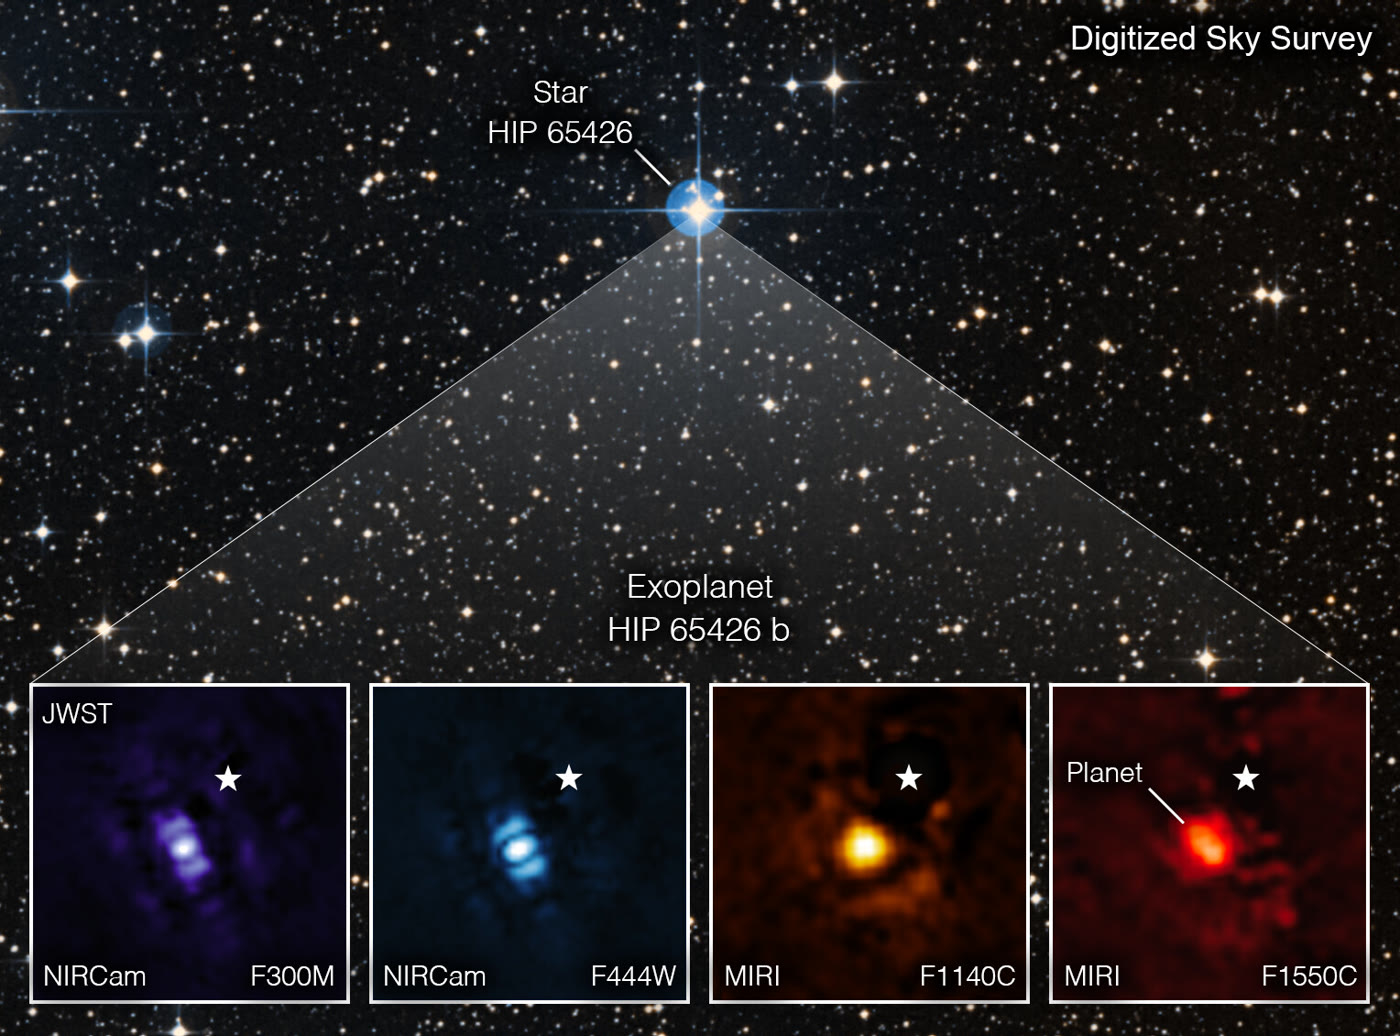
\includegraphics[width=0.86\linewidth]{images/book5/b3-hip65426b.jpg}
\par\smallskip{\small La première exoplanète imagée par le James Webb Space
Telescope, HIP~65426~b, dans quatre filtres infrarouges (en bas~; en haut, le
champ de l'étoile dans un relevé du ciel depuis le sol)~; la lumière de
l'étoile, à la position du symbole d'étoile, est bloquée par les
\omterm{def:b3:exoplanets:imaging}{coronographes}. La planète est une jeune géante gazeuse d'environ 6 à 8 masses de
Jupiter, âgée de quelque 15 à 20 millions d'années, située à environ cent
fois plus loin de son étoile que la Terre ne l'est du Soleil. Image NASA/ESA/CSA,
A~Carter (UCSC), l'équipe ERS~1386 et A.~Pagan (STScI), CC
BY~4.0.}\label{fig:b3:exoplanets:hip65426}
\end{omfigure}
% ledger: photo:b3-hip65426b

Une quatrième méthode utilise la gravité comme une lentille. Lorsqu'une étoile passe presque exactement
devant une étoile plus lointaine, sa gravité courbe la lumière de l'étoile
d'arrière-plan et la rend plus brillante pendant quelques semaines~; une planète de l'étoile
qui fait office de lentille ajoute un bref signal.

\begin{definition}[Microlentille gravitationnelle~; rayon d'Einstein]\label{def:b3:exoplanets:microlensing}
La \emph{microlentille gravitationnelle}\index{microlentille gravitationnelle} désigne
l'éclaircissement temporaire d'une étoile d'arrière-plan lorsqu'une étoile de premier plan,
la lentille, passe près de la ligne de visée~; les images qu'elle forme sont trop proches
pour être résolues. Le \emph{rayon d'Einstein}\index{rayon d'Einstein} est le rayon angulaire
$\theta_\mathrm E$ de l'anneau dans lequel une lentille ponctuelle
de masse $M$ située à la distance $D_L$ ferait converger une source située à la
distance $D_S$ exactement derrière elle~:
\[
\theta_\mathrm E = \sqrt{\frac{4GM}{c^2}\,\frac{D_S - D_L}{D_L D_S}} .
\]
\end{definition}

\begin{proposition}[Grandissement d'une lentille ponctuelle]\label{prop:b3:exoplanets:magnification}
Une source située à la distance angulaire $u\,\theta_\mathrm E$ d'une lentille ponctuelle
est éclaircie d'un facteur
\[
A(u) = \frac{u^2 + 2}{u\sqrt{u^2 + 4}} .
\]
\end{proposition}

\admitted

Ces deux résultats proviennent de la déviation de la lumière par une masse en relativité générale.
Pour une lentille d'une demi-masse solaire située à mi-chemin d'une source
distante de \qty{8}{kpc}, on a $\theta_\mathrm E = \qty{0.71}{mas}$, et l'anneau d'Einstein
à la distance de la lentille, a un rayon de \qty{2.9}{au}.
Pour $u = 1$, la source est éclaircie 1.34 fois~; pour $u = 0.1$, dix fois. Une
planète proche de l'anneau d'Einstein de son étoile ajoute une courte déviation à la
courbe de lumière. La microlentille permet ainsi de détecter des planètes à quelques
unités astronomiques de leur étoile, des planètes froides qui échappent aux \omterm{def:b3:exoplanets:transit}{méthodes
des transits} et des vitesses radiales, mais chaque événement ne survient qu'une fois et ne se répète jamais. Lors d'un événement de 2003,
publié l'année suivante, une déviation d'une durée d'environ sept jours n'a pu être expliquée que
par un compagnon dont la masse vaut $\num{0.0039}$ fois celle de la lentille~: une planète
d'environ 1.5 fois la masse de Jupiter, à environ \qty{3}{au} de son
étoile.
% ledger: const:G, const:c, sun:mass, iau:parsec, const:au, bond04:ogle235

\begin{omfigure}
\centering
\begin{tikzpicture}[scale=0.95]
\fill (0,0) circle (0.06) node[below=2pt, font=\scriptsize] {source};
\fill[omDef] (3.2,0) circle (0.09); \node[font=\scriptsize, omDef] at (3.2,-1.15) {lentille};
\draw[omDef] (3.2,0) ellipse (0.12 and 0.9);
\fill (6.4,0) circle (0.06) node[below=2pt, font=\scriptsize] {observateur};
\draw[thick, orange!80!black] (0,0) -- (3.2,0.9) -- (6.4,0);
\draw[thick, orange!80!black] (0,0) -- (3.2,-0.9) -- (6.4,0);
\draw[densely dashed, black!50] (6.4,0) -- (0,1.8) node[left, font=\scriptsize] {image};
\draw[densely dotted, black!50] (0,0) -- (6.4,0);
\draw[<->] (3.55,0) -- (3.55,0.9) node[midway, right, font=\scriptsize] {$R_\mathrm E$};
\draw[<->, black!60] (0,-1.5) -- (3.2,-1.5) node[midway, below, font=\scriptsize] {$D_S - D_L$};
\draw[<->, black!60] (3.2,-1.5) -- (6.4,-1.5) node[midway, below, font=\scriptsize] {$D_L$};
\end{tikzpicture}\hfill
\begin{tikzpicture}
\begin{axis}[width=0.48\linewidth, height=0.42\linewidth,
  xmin=-3, xmax=3, ymin=0.8, ymax=12, ymode=log,
  ytick={1,2,5,10}, yticklabels={1,2,5,10},
  xlabel={temps ($t_\mathrm E$)}, ylabel={grandissement $A$},
  tick label style={font=\scriptsize}, label style={font=\small},
  legend style={font=\scriptsize, at={(0.5,-0.30)}, anchor=north, legend columns=3, draw=none, cells={anchor=west}, /tikz/every even column/.append style={column sep=1em}}]
\addplot[thick, omDef] table[x=t_tE, y=A01] {figdata/out/bachelor-3-rv_transit-lens.dat};
\addlegendentry{$u_0 = 0.1$}
\addplot[thick, dashed, red!70!black] table[x=t_tE, y=A03] {figdata/out/bachelor-3-rv_transit-lens.dat};
\addlegendentry{$0.3$}
\addplot[thick, dotted, black] table[x=t_tE, y=A10] {figdata/out/bachelor-3-rv_transit-lens.dat};
\addlegendentry{$1$}
\end{axis}
\end{tikzpicture}
\par\smallskip{\small À gauche~: la géométrie d'une lentille gravitationnelle, non à
l'échelle~; les rayons issus de la source passent près de la lentille, à environ un \omterm{def:b3:exoplanets:microlensing}{rayon d'Einstein}
$R_\mathrm E = \theta_\mathrm E D_L$ et atteignent l'observateur, qui voit la
source décalée vers l'image. À droite~: le grandissement d'une source ponctuelle
par une lentille ponctuelle en fonction du temps, en unités du temps $t_\mathrm E$ que
met la lentille pour se déplacer d'un \omterm{def:b3:exoplanets:microlensing}{rayon d'Einstein}, pour trois distances minimales
d'approche $u_0$ (en \omterm{def:b3:exoplanets:microlensing}{rayons d'Einstein}).}\label{fig:b3:exoplanets:microlensing}
\end{omfigure}

Chaque méthode a ses propres biais, et le catalogue des planètes connues
les reflète. Les vitesses radiales favorisent les planètes massives proches de leur étoile~;
les transits favorisent les planètes de grande taille proches de leur étoile, et exigent
que l'orbite soit vue de profil~; la microlentille détecte les planètes situées à quelques unités astronomiques~;
l'imagerie détecte les jeunes géantes à des dizaines ou des centaines d'unités astronomiques de leur étoile.
La figure ci-dessous montre le résultat~: chaque méthode couvre sa propre région, et
les planètes du Système solaire se trouvent pour la plupart dans les lacunes qui les séparent.

\begin{dated}{2026}
Le 23 octobre 2026, la NASA Exoplanet Archive recensait 6451 exoplanètes confirmées.
Par méthode de découverte~: 4785 par transits, 1204 par vitesses radiales,
292 par microlentille, 98 par imagerie, 29 par \omterm{def:b3:exoplanets:ttv}{variations du temps de transit} (TTV)
et le reste par des méthodes plus rares, parmi lesquelles les toutes premières,
découvertes en 1992 autour d'un pulsar grâce au chronométrage de ses impulsions.
Les premières découvertes par vitesses radiales datent de 1995, par transit de 2002, par
microlentille et imagerie à partir de 2004.
\end{dated}
% ledger: data:b5-pscomp

\begin{omfigure}
\centering
\begin{tikzpicture}
\begin{axis}[width=0.86\linewidth, height=0.56\linewidth,
  xmode=log, ymode=log, xmin=0.004, xmax=2000, ymin=0.02, ymax=1e5,
  legend image post style={scale=2.2},
  xlabel={demi-grand axe (au)}, ylabel={masse ou masse minimale ($M_\oplus$)},
  tick label style={font=\scriptsize}, label style={font=\small},
  legend style={font=\scriptsize, at={(0.5,-0.20)}, anchor=north, legend columns=4, draw=none, cells={anchor=west}, /tikz/every even column/.append style={column sep=1em}}]
\addplot[only marks, mark=*, mark size=0.6pt, omDef, opacity=0.6] table[x=a_au, y=mass] {figdata/out/bachelor-3-exoplanet_archive-ma-tr.dat};
\addlegendentry{transit}
\addplot[only marks, mark=*, mark size=0.6pt, red!70!black, opacity=0.6] table[x=a_au, y=mass] {figdata/out/bachelor-3-exoplanet_archive-ma-rv.dat};
\addlegendentry{vitesse radiale}
\addplot[only marks, mark=triangle*, mark size=1.2pt, green!45!black] table[x=a_au, y=mass] {figdata/out/bachelor-3-exoplanet_archive-ma-ml.dat};
\addlegendentry{microlentille}
\addplot[only marks, mark=diamond*, mark size=1.5pt, orange!85!black] table[x=a_au, y=mass] {figdata/out/bachelor-3-exoplanet_archive-ma-im.dat};
\addlegendentry{imagerie}
\addplot[only marks, mark=square*, mark size=1.6pt, black, forget plot] table[x=a_au, y=mass] {figdata/out/bachelor-3-exoplanet_archive-solar.dat};
\node[font=\scriptsize, anchor=west, fill=white, inner sep=1pt] at (axis cs:1.15,1.0) {Terre};
\node[font=\scriptsize, anchor=east, fill=white, inner sep=1pt] at (axis cs:0.63,0.82) {Vénus};
\node[font=\scriptsize, anchor=east, fill=white, inner sep=1pt] at (axis cs:0.34,0.055) {Mercure};
\node[font=\scriptsize, anchor=west, fill=white, inner sep=1pt] at (axis cs:1.75,0.107) {Mars};
\node[font=\scriptsize, anchor=west, fill=white, inner sep=1pt] at (axis cs:6.0,318) {Jupiter};
\node[font=\scriptsize, anchor=west, fill=white, inner sep=1pt] at (axis cs:11,95) {Saturne};
\node[font=\scriptsize, anchor=north, fill=white, inner sep=1pt] at (axis cs:25,11) {Uranus, Neptune};
\end{axis}
\end{tikzpicture}
\par\smallskip{\small Planètes confirmées dont on connaît la masse (ou la \omterm{def:b3:exoplanets:rv}{masse minimale})
et le demi-grand axe, réparties par méthode de découverte (NASA Exoplanet
Archive, 23 octobre 2026~: 1691 par transit, 1151 par vitesses radiales, 286
par microlentille, 94 par imagerie), avec les planètes du Système solaire (carrés
noirs). Les masses prédites à partir d'une \omterm{def:b3:exoplanets:mass-radius}{relation masse--rayon} sont exclues. Cette recherche
a utilisé la NASA Exoplanet Archive, qui est exploitée par le
California Institute of Technology, dans le cadre d'un contrat avec la National
Aeronautics and Space Administration, au titre du programme Exoplanet
Exploration Program.}\label{fig:b3:exoplanets:methods}
\end{omfigure}
% ledger: data:b5-pscomp, planet:Mercury.mass, planet:Venus.mass, planet:Earth.mass, planet:Mars.mass, planet:Jupiter.mass, planet:Saturn.mass, planet:Uranus.mass, planet:Neptune.mass, planet:Mercury.dist, planet:Venus.dist, planet:Earth.dist, planet:Mars.dist, planet:Jupiter.dist, planet:Saturn.dist, planet:Uranus.dist, planet:Neptune.dist

\section{Ce qui a été trouvé}\label{sec:b3:exoplanets:found}

La première surprise fut celle des \omterm{def:b3:exoplanets:classes}{Jupiter chauds}, des planètes géantes sur des orbites de
quelques jours. 51~Pegasi~b ne peut pas s'être formée si près de son étoile~; elle a dû
se former plus loin, peut-être à quelques unités astronomiques, au-delà de la ligne des
glaces de son disque, puis migrer vers l'intérieur par son interaction avec le disque,
comme la théorie l'avait prédit.
% ledger: nobel19:migration

\begin{definition}[Jupiter chaud~; super-Terre~; sous-Neptune]\label{def:b3:exoplanets:classes}
Un \emph{Jupiter chaud}\index{Jupiter chaud} est une planète géante sur une orbite serrée,
dont la \omterm{def:b3:exoplanets:rv}{masse minimale} est généralement supérieure à 0.1 masse de Jupiter et dont la période
est inférieure à dix jours. Une \emph{super-Terre}\index{super-Terre} est une planète plus grande
que la Terre mais plus petite que la \omterm{def:b3:exoplanets:radius-valley}{vallée des rayons}, soit jusqu'à environ 1.5 à 2 rayons
terrestres, et donc probablement rocheuse. Un \emph{sous-Neptune}\index{sous-Neptune}
est une planète située au-dessus de la \omterm{def:b3:exoplanets:radius-valley}{vallée des rayons} mais plus petite que Neptune, d'environ 2
à 4 rayons terrestres, dont le rayon suppose une enveloppe de gaz légers ou de
composés volatils.
\end{definition}
% ledger: wright12:hj, fulton17:gap, planet:Neptune.diameter, planet:Earth.diameter

\begin{definition}[Taux d'occurrence]\label{def:b3:exoplanets:occurrence}
Le \emph{taux d'occurrence}\index{taux d'occurrence} d'une classe de planètes est le
nombre moyen de telles planètes par étoile, ou la fraction d'étoiles en possédant une,
dans un intervalle donné de taille (ou de masse) et de période, une fois les comptages d'un
relevé corrigés des planètes qu'il n'a pas pu détecter~: celles dont les orbites ne sont
pas alignées pour un transit, et celles qui sont trop petites ou trop éloignées pour être
vues.
\end{definition}

Les \omterm{def:b3:exoplanets:classes}{Jupiter chauds}, très présents dans le catalogue parce qu'ils sont les plus faciles à
trouver, sont rares~: un relevé par vitesses radiales d'étoiles voisines semblables au Soleil
en a trouvé autour de \qty[separate-uncertainty=true]{1.2 \pm 0.38}{\percent} des étoiles. Les petites planètes sont
courantes. En exploitant les courbes de lumière de \num{42000} étoiles observées par le
télescope spatial Kepler, une étude a trouvé 603 planètes, dont dix de la taille de la Terre (1 à 2
rayons terrestres) recevant entre une et quatre fois l'éclairement solaire terrestre~; une fois
corrigé de la probabilité de transit et des planètes que la recherche aurait manquées,
\qty[separate-uncertainty=true]{11 \pm 4}{\percent} des étoiles semblables au Soleil en abritent une telle
planète.
% ledger: wright12:hj, petigura13:eta

La taille des petites planètes n'est pas répartie uniformément. Parmi les planètes proches
de leur étoile mesurées avec précision, celles de 1.5 à 2.0 rayons terrestres sont au
moins deux fois plus rares que celles juste un peu plus petites ou juste un peu plus grandes.

\begin{definition}[Vallée des rayons]\label{def:b3:exoplanets:radius-valley}
La \emph{vallée des rayons}\index{vallée des rayons} est le déficit de planètes
de rayons compris entre environ 1.5 et 2.0 rayons terrestres parmi les planètes
de périodes inférieures à une centaine de jours~; elle sépare les \omterm{def:b3:exoplanets:classes}{super-Terres}
des \omterm{def:b3:exoplanets:classes}{sous-Neptunes}.
\end{definition}
% ledger: fulton17:gap

La vallée est interprétée comme la trace de l'échappement. Un noyau rocheux formé avec une
enveloppe d'hydrogène et d'hélium ne représentant que quelques pour cent de sa masse a un
rayon deux fois supérieur à celui du noyau nu. Près d'une jeune étoile active, une telle
enveloppe est chauffée puis perdue par \omterm{def:b3:planetary-atmospheres:hydrodynamic}{échappement hydrodynamique}~: sous l'effet du
rayonnement de haute énergie de l'étoile pendant les cent premiers millions d'années
(photoévaporation), ou sous celui de la chaleur du noyau lui-même en refroidissement
(perte de masse alimentée par le noyau). Les modèles regroupent les planètes en noyaux nus
d'environ 1.3 rayon terrestre et en planètes deux fois plus grandes~; peu en subsistent
entre les deux. Les deux mécanismes dépendent différemment de l'étoile, et des planètes
autour d'étoiles de types différents pourraient permettre de les distinguer.
% ledger: owen17:valley, ginzburg18:core-powered

\begin{omfigure}
\centering
\begin{tikzpicture}
\begin{axis}[name=pr, width=0.50\linewidth, height=0.50\linewidth,
  xmode=log, ymode=log, xmin=1, xmax=100, ymin=0.8, ymax=4,
  ytick={1,1.5,2,3,4}, yticklabels={1,1.5,2,3,4},
  xlabel={période (jours)}, ylabel={rayon ($R_\oplus$)},
  tick label style={font=\scriptsize}, label style={font=\small},
  title={(a)}, title style={font=\small}]
\fill[black!10] (axis cs:1,1.5) rectangle (axis cs:100,2.0);
\addplot[only marks, mark=*, mark size=0.5pt, omDef, opacity=0.7] table[x=period, y=radius] {figdata/out/bachelor-3-exoplanet_archive-pr.dat};
\end{axis}
\begin{axis}[at={(pr.east)}, anchor=west, xshift=0.09\linewidth,
  width=0.42\linewidth, height=0.50\linewidth,
  xmode=log, xmin=0.8, xmax=4, ymin=0, ymax=185,
  xtick={1,1.5,2,3,4}, xticklabels={1,1.5,2,3,4},
  xlabel={rayon ($R_\oplus$)}, ylabel={nombre de planètes},
  tick label style={font=\scriptsize}, label style={font=\small},
  title={(b)}, title style={font=\small}]
\fill[black!10] (axis cs:1.5,0) rectangle (axis cs:2.0,185);
\addplot[const plot mark left, thick, omDef, fill=omDef!25] table[x=r, y=n] {figdata/out/bachelor-3-exoplanet_archive-histstep.dat} \closedcycle;
\end{axis}
\end{tikzpicture}
\par\smallskip{\small (a)~Planètes en transit dont le rayon est connu à mieux que
\qty{10}{\percent} près, autour d'étoiles de rayon inférieur à deux rayons solaires, de
périodes de 1 à 100 jours (2370 planètes, NASA Exoplanet Archive, 23
octobre 2026)~; en grisé, la \omterm{def:b3:exoplanets:radius-valley}{vallée des rayons} de 1.5 à 2.0 rayons terrestres.
(b)~Les mêmes planètes comptées dans 20 intervalles de largeur égale en $\log R$.
Les comptages ne sont pas corrigés des planètes que les relevés manquent, celles-ci étant
plus nombreuses parmi les petites~; la vallée apparaît néanmoins.}\label{fig:b3:exoplanets:valley}
\end{omfigure}
% ledger: data:b5-pscomp, fulton17:gap

\begin{definition}[Relation masse--rayon]\label{def:b3:exoplanets:mass-radius}
La \emph{relation masse--rayon}\index{relation masse--rayon} d'une composition est le rayon
d'une planète de cette composition en fonction de sa masse,
calculé à partir des équations d'état de ses matériaux en
équilibre hydrostatique~; une planète mesurée est comparée aux
relations des compositions candidates.
\end{definition}

Une planète rocheuse est comprimée par son propre poids, et son rayon croît
plus lentement que $M^{1/3}$. Un ajustement sur des modèles de planètes à deux couches construits
à partir du modèle sismique terrestre donne $R/R_\oplus = (1.07 - 0.21\,C)
(M/M_\oplus)^{1/3.7}$, pour des masses de 1 à 8 masses terrestres et une fraction
massique de noyau $C$ de 0 à 0.4~; ajusté à la Terre, à Vénus et à quelques petites
exoplanètes, il donne $C = 0.26 \pm 0.07$. Une
planète de fer est plus petite à même masse~; une planète moitié eau, plus grande~;
une enveloppe d'hydrogène de seulement deux pour cent de la masse fait d'une planète de
cinq masses terrestres une planète de \num{2.6} rayons terrestres, à la taille d'un
\omterm{def:b3:exoplanets:classes}{sous-Neptune}. La dégénérescence est réelle~: un rayon et une masse donnent une seule
masse volumique, et plusieurs mélanges de fer, de roche, d'eau et de gaz peuvent la partager.
La planète rocheuse Kepler-10~b, de 3.24 masses terrestres et 1.47 rayon terrestre,
a une masse volumique moyenne de \qty{5.6}{g.cm^{-3}}~; la géante gazeuse WASP-39~b,
de 89 masses terrestres et 14.3 rayons terrestres, \qty{0.17}{g.cm^{-3}}.
% ledger: zeng16:rocky, data:b5-zeng, data:b5-pscomp

\begin{omfigure}
\centering
\begin{tikzpicture}
\begin{axis}[width=0.86\linewidth, height=0.58\linewidth,
  xmode=log, ymode=log, xmin=0.3, xmax=5000, ymin=0.5, ymax=25,
  ytick={0.5,1,2,4,10,20}, yticklabels={0.5,1,2,4,10,20},
  xlabel={masse ($M_\oplus$)}, ylabel={rayon ($R_\oplus$)},
  tick label style={font=\scriptsize}, label style={font=\small},
  legend style={font=\scriptsize, at={(0.5,-0.20)}, anchor=north, legend columns=3, draw=none, cells={anchor=west}, /tikz/every even column/.append style={column sep=1em}}]
\addplot[only marks, mark=*, mark size=0.6pt, black!35, forget plot] table[x=mass, y=radius] {figdata/out/bachelor-3-exoplanet_archive-mr.dat};
\addplot[thick, black] table[x=mass, y=radius] {figdata/out/bachelor-3-exoplanet_archive-zeng-iron.dat};
\addlegendentry{fer pur}
\addplot[thick, brown!70!black] table[x=mass, y=radius] {figdata/out/bachelor-3-exoplanet_archive-zeng-earthlike.dat};
\addlegendentry{roche de type terrestre}
\addplot[thick, omDef] table[x=mass, y=radius] {figdata/out/bachelor-3-exoplanet_archive-zeng-water50.dat};
\addlegendentry{50\,\% d'eau}
\addplot[thick, dashed, orange!85!black] table[x=mass, y=radius] {figdata/out/bachelor-3-exoplanet_archive-zeng-h2-2pc.dat};
\addlegendentry{roche + 2\,\% d'hydrogène}
\addplot[only marks, mark=square*, mark size=1.8pt, red!70!black] table[x=mass, y=radius] {figdata/out/bachelor-3-exoplanet_archive-solar.dat};
\addlegendentry{Système solaire}
\node[font=\scriptsize, anchor=north west] at (axis cs:1.05,0.97) {Terre};
\node[font=\scriptsize, anchor=south east] at (axis cs:0.80,0.97) {Vénus};
\node[font=\scriptsize, anchor=south east, fill=white, inner sep=1pt] at (axis cs:13.5,4.3) {Uranus, Neptune};
\node[font=\scriptsize, anchor=east, fill=white, inner sep=1pt] at (axis cs:80,9.45) {Saturne};
\node[font=\scriptsize, anchor=north, fill=white, inner sep=1pt] at (axis cs:318,10.3) {Jupiter};
\end{axis}
\end{tikzpicture}
\par\smallskip{\small Masse et rayon de 1078 planètes en transit dont la
masse est mesurée à mieux de \qty{25}{\percent} et le rayon à mieux de
\qty{10}{\percent} (en gris~; NASA Exoplanet Archive, 23 octobre 2026),
avec les courbes de modèles de L.~Zeng et al. (2016, 2019)~: fer pur~;
roche de type terrestre, un tiers de fer et deux tiers de silicates~; moitié
d'eau sur un tel noyau, à \qty{500}{K}~; un noyau de type terrestre avec une
enveloppe d'hydrogène de \qty{2}{\percent} de sa masse, à \qty{500}{K}. Carrés
rouges~: les planètes du Système solaire (Mercure et Mars se trouvent hors de
l'échelle, à gauche).}\label{fig:b3:exoplanets:mass-radius}
\end{omfigure}
% ledger: data:b5-pscomp, data:b5-zeng, planet:Earth.mass, planet:Earth.diameter, planet:Venus.mass, planet:Venus.diameter, planet:Jupiter.mass, planet:Jupiter.diameter, planet:Saturn.mass, planet:Saturn.diameter, planet:Uranus.mass, planet:Uranus.diameter, planet:Neptune.mass, planet:Neptune.diameter

\section{Atmosphères}\label{sec:b3:exoplanets:atmospheres}

Une planète en transit peut être pesée et mesurée~; on peut aussi la sentir.
Pendant un transit, un mince anneau de l'atmosphère de la planète se détache
devant l'étoile, et la lumière stellaire le traverse. Aux longueurs
d'onde où un gaz de l'atmosphère absorbe, l'anneau est opaque plus haut, et
la planète paraît plus grande.

\begin{definition}[Spectroscopie de transmission~; éclipse secondaire]\label{def:b3:exoplanets:transmission}
La \emph{spectroscopie de transmission}\index{spectroscopie de transmission} mesure
la \omterm{def:b3:exoplanets:transit}{profondeur de transit} en fonction de la longueur d'onde, afin de détecter les
gaz de l'atmosphère que la lumière stellaire traverse au bord de la planète. Une
\emph{éclipse secondaire}\index{eclipse@éclipse secondaire} est le passage d'une
planète derrière son étoile, une demi-orbite après le transit sur une orbite
circulaire~; la baisse du flux du système mesure alors la lumière de la
face diurne de la planète.
\end{definition}

\begin{proposition}[Signal de transmission]\label{prop:b3:exoplanets:transmission}
Une atmosphère de hauteur d'échelle $H \ll R_p$, rendue opaque sur $n$ hauteurs
d'échelle supplémentaires à la longueur d'onde d'une bande d'absorption plutôt
qu'aux longueurs d'onde voisines, approfondit là le transit de
\[
\Delta\delta \approx n\,\frac{2HR_p}{R_\star^2} .
\]
\end{proposition}

\begin{proof}
Le rayon apparent de la planète passe de $R_p$ à $R_p + nH$, de sorte que la
profondeur $(R_p + nH)^2/R_\star^2$ croît de $(2nHR_p + n^2H^2)/R_\star^2$,
soit $2nHR_p/R_\star^2$ lorsque $nH \ll R_p$.
\end{proof}

La hauteur d'échelle $H = kT/\bar m g$ est grande pour une planète chaude de
faible pesanteur, dotée d'un air léger à base d'hydrogène~; elle est petite pour
une planète froide et dense, à air lourd. Pour la Terre vue devant le Soleil, avec
$H = \qty{8}{km}$, chaque hauteur d'échelle ajoute 0.2 partie par million~; pour une
géante gazeuse chaude et gonflée, plusieurs centaines.
% ledger: planet:Earth.diameter, sun:R

\begin{proposition}[Profondeur de l'éclipse secondaire]\label{prop:b3:exoplanets:eclipse}
Si la face diurne d'une planète rayonne comme un corps noir à la température
$T_d$ et l'étoile comme un corps noir à $T_\star$, l'\omterm{def:b3:exoplanets:transmission}{éclipse secondaire} à la
longueur d'onde $\lambda$ a pour profondeur
\[
\delta_\mathrm{ecl} \approx \left(\frac{R_p}{R_\star}\right)^2
  \frac{B_\lambda(T_d)}{B_\lambda(T_\star)},
\]
avec $B_\lambda$ la loi de Planck, la lumière réfléchie par la planète étant négligée.
\end{proposition}

\begin{proof}
Juste avant l'éclipse, l'observateur reçoit la lumière de l'étoile, proportionnelle à
$\pi R_\star^2 B_\lambda(T_\star)$, plus celle de la face diurne, proportionnelle à
$\pi R_p^2 B_\lambda(T_d)$~; pendant l'éclipse, seule celle de l'étoile. La baisse
fractionnaire est le rapport entre le terme de la planète et celui de l'étoile,
le premier étant petit.
\end{proof}

L'éclipse est la plus profonde dans l'infrarouge, où la planète froide est la plus
brillante par rapport à son étoile~: elle donne la température de la face diurne, et
une face diurne chaude à côté d'une face nocturne froide révèle une atmosphère mince
ou absente, qui ne fait pas circuler la chaleur.

\begin{dated}{2023}
En 2022, le spectre de transmission de la géante gazeuse WASP-39~b, mesuré
entre 3.0 et \qty{5.5}{\micro m} par le télescope spatial James Webb,
a montré une bande d'absorption marquée du dioxyde de carbone à
\qty{4.3}{\micro m}, à 26 écarts types, là où la photométrie antérieure
n'avait fait qu'entrevoir le gaz~: sa première identification nette dans
l'atmosphère d'une exoplanète. En 2023, cinq \omterm{def:b3:exoplanets:transmission}{éclipses secondaires} de
TRAPPIST-1~b, de la taille de la Terre, qui reçoit quatre fois la lumière que reçoit la
Terre, venant d'une étoile froide et petite, ont été mesurées à \qty{15}{\micro m}. Elles
s'accordent avec une chaleur réémise par la seule face diurne, sans
dioxyde de carbone détectable~: la planète a peu ou pas d'atmosphère pour
transporter la chaleur vers sa face nocturne.
\end{dated}
% ledger: jwst23:wasp39-co2, greene23:trappist1b

Les planètes rocheuses des zones habitables des petites étoiles sont à portée
de ces méthodes, à la limite. Savoir si elles ont conservé leur air face aux
processus d'échappement du chapitre précédent est désormais une question
observationnelle.

\section{Exercices}

\begin{exercise}[$\star$]\label{exo:b3:exoplanets:1}
(a)~Calculer l'amplitude semi-majeure de la vitesse radiale du Soleil causée par
Jupiter (masse \qty{1898e24}{kg}, période \num{4331}~jours, excentricité
0.049) et par la Terre (masse \qty{5.97e24}{kg}, période \num{365.2}~jours,
excentricité 0.017). La masse du Soleil est \qty{1.9884e30}{kg}.
(b)~Convertir les précisions \qty{3.5}{km/h} et \qty{0.35}{km/h} en
mètres par seconde, puis comparer.
\end{exercise}

\begin{exercise}[$\star$]\label{exo:b3:exoplanets:2}
(a)~Calculer les \omterm{def:b3:exoplanets:transit}{profondeurs de transit} de Jupiter (rayon \qty{71492}{km}) et de
la Terre (rayon \qty{6378}{km}) devant le Soleil (rayon
\qty{695700}{km}). (b)~Calculer la probabilité qu'un observateur placé au hasard
voie chacune d'elles transiter, pour des rayons orbitaux de \num{778.5}
et \qty{149.6}{\mega km}.
\end{exercise}

\begin{exercise}[$\star$]\label{exo:b3:exoplanets:3}
51~Pegasi~b donne à son étoile une amplitude semi-majeure de la vitesse radiale de
\qty{59}{m.s^{-1}}, avec une période de \qty{4.23}{d}. En prenant la masse de
l'étoile égale à celle du Soleil, calculer la \omterm{def:b3:exoplanets:rv}{masse minimale} de la planète, en
masses de Jupiter et en masses terrestres, ainsi que le rayon de son orbite.
\end{exercise}

\begin{exercise}[$\star$]\label{exo:b3:exoplanets:4}
Une étoile de demi-masse solaire située à \qty{4}{kpc} agit comme lentille sur une
étoile située à \qty{8}{kpc} ($\qty{1}{pc} = \qty{3.0857e16}{m}$). (a)~Calculer
son \omterm{def:b3:exoplanets:microlensing}{rayon d'Einstein} en millisecondes d'arc, ainsi que le rayon de l'anneau
d'Einstein, en unités astronomiques, à la distance de la lentille. (b)~Calculer
l'amplification pour $u = 1$, $0.5$ et $0.1$. (c)~Combien de temps la lentille
met-elle pour parcourir un \omterm{def:b3:exoplanets:microlensing}{rayon d'Einstein} si elle se déplace dans la ligne de
visée à \qty{200}{km.s^{-1}}~?
\end{exercise}

\begin{exercise}[$\star\star$]\label{exo:b3:exoplanets:5}
Une planète de rapport de rayons $p = 0.12$ orbite autour d'une étoile d'une
masse et d'un rayon solaires en \qty{3.0}{d}. (a)~Calculer $a/R_\star$. (b)~Calculer
$T_{14}$ et $T_{23}$ pour $b = 0$ et pour $b = 0.7$, ainsi que l'inclinaison
dans le second cas. (c)~En quoi la forme de la courbe de lumière permet-elle de
distinguer un transit central d'un transit rasant~?
\end{exercise}

\begin{exercise}[$\star\star$]\label{exo:b3:exoplanets:6}
À partir des masses et des rayons de l'Exoplanet Archive, calculer les masses
volumiques moyennes de TRAPPIST-1~b (1.374 masse terrestre, 1.116 rayon
terrestre), Kepler-10~b (3.24, 1.47), WASP-39~b (89.31, 14.34) et
HD~209458~b (232.0, 15.58), avec $M_\oplus = \qty{5.97e24}{kg}$ et $R_\oplus =
\qty{6378}{km}$. Lesquelles sont rocheuses, lesquelles sont gazeuses~?
\end{exercise}

\begin{exercise}[$\star\star$]\label{exo:b3:exoplanets:7}
La vitesse radiale d'une étoile accompagnée d'une planète sur une orbite excentrique
varie de $+\qty{50.4}{m.s^{-1}}$ à $-\qty{9.6}{m.s^{-1}}$, et la vitesse du centre
de masse du système vaut \qty{12.4}{m.s^{-1}}. En utilisant la forme excentrique du
théorème, calculer $K$ et $e\cos\omega$. Pourquoi la moyenne des deux valeurs
extrêmes peut-elle différer de $\gamma$~?
\end{exercise}

\begin{exercise}[$\star\star$]\label{exo:b3:exoplanets:8}
WASP-39~b a une masse de 89.31 masses terrestres et un rayon de 14.34 rayons
terrestres~; son étoile a un rayon de 0.939 rayon solaire. Prendre une température de
\qty{1100}{K} et une masse moléculaire moyenne de \qty{2.3}{u} pour son atmosphère.
(a)~Calculer sa gravité, sa hauteur d'échelle et sa \omterm{def:b3:exoplanets:transit}{profondeur de transit}.
(b)~Calculer le signal de transmission d'une hauteur d'échelle, puis celui d'une
bande d'absorption haute de deux hauteurs d'échelle, en parties par million.
\end{exercise}

\begin{exercise}[$\star\star$]\label{exo:b3:exoplanets:9}
TRAPPIST-1~b a un rayon de 1.116 rayon terrestre~; son étoile, un rayon de 0.1192
rayon solaire et une température de \qty{2566}{K}. Calculer la profondeur de son
\omterm{def:b3:exoplanets:transmission}{éclipse secondaire} à \qty{15}{\micro m} pour un côté jour à \qty{400}{K}, puis à
\qty{500}{K} ($hc/k = \qty{0.014388}{m.K}$). Pourquoi une mesure de la profondeur
constitue-t-elle un thermomètre~?
\end{exercise}

\begin{exercise}[$\star\star\star$]\label{exo:b3:exoplanets:10}
Une naine rouge fictive a une masse de 0.2 masse solaire, un rayon de 0.2 rayon
solaire et une luminosité de \num{0.005} luminosité solaire. (a)~À quelle distance
une planète reçoit-elle le flux stellaire terrestre, et quelle est sa période~?
(b)~Calculer l'amplitude semi-majeure causée par une planète d'une masse terrestre
à cette distance, et la comparer à l'effet de la Terre sur le Soleil. (c)~Calculer la
\omterm{def:b3:exoplanets:transit}{profondeur de transit} d'une planète de la taille de la Terre. Pourquoi de tels
astres sont-ils des cibles privilégiées dans la recherche de planètes rocheuses en zone habitable~?
\end{exercise}

\begin{exercise}[$\star\star\star$]\label{exo:b3:exoplanets:11}
Pour la loi quadratique d'\omterm{def:b3:exoplanets:limb}{assombrissement centre-bord}, montrer que l'intensité
moyenne du disque vaut $I(1)(1 - u_1/3 - u_2/6)$. En déduire la profondeur, en unités
de $p^2$, d'une petite planète en $r = 0$, $0.5$ et $0.9$ pour $u_1 = 0.40$,
$u_2 = 0.25$. Quelle erreur un modèle à disque uniforme commettrait-il sur le rayon
d'une planète observée à mi-transit avec $b = 0$~?
\end{exercise}

\begin{exercise}[$\star\star\star$]\label{exo:b3:exoplanets:12}
Une étude a suivi \num{42000} étoiles semblables au Soleil et y a recherché des planètes
de la taille de la Terre recevant de un à quatre fois le flux solaire terrestre,
c'est-à-dire sur des orbites de 0.5 à \qty{1}{au}. (a)~Calculer la probabilité de
transit à 0.5, 0.7 et \qty{1}{au}. (b)~Si \qty{11}{\percent} des étoiles
hébergent une telle planète, à environ \qty{0.7}{au}, combien transitent~?
(c)~L'étude en a trouvé dix. Que mesure l'écart, et pourquoi le \omterm{def:b3:exoplanets:occurrence}{taux d'occurrence}
doit-il être corrigé de celui-ci~?
\end{exercise}

\section{Problème~: la lampe de Séléné}

\begin{problem}[{Problème du week-end --- pesée, dimensionnement et analyse
d'une planète inventée}]
\label{pb:b3:exoplanets:1}
La lampe de Séléné est une naine~K inventée, de masse égale à 0.80 fois celle du Soleil, de rayon
0.76 fois celui du Soleil et de température effective \qty{5000}{K}. Une
étude par la \omterm{def:b3:exoplanets:rv}{méthode des vitesses radiales} établit que sa vitesse varie sinusoïdalement avec
une période de \qty{12.0}{d} et une semi-amplitude de \qty{2.59}{m.s^{-1}}. Un
télescope spatial observe alors des transits de même période, de profondeur
\num{838} parties par million et de durée totale $T_{14} = \qty{3.23}{h}$.
Prendre $M_\odot = \qty{1.9884e30}{kg}$, $R_\odot = \qty{695700}{km}$,
$L_\odot = \qty{3.828e26}{W}$, $M_\oplus = \qty{5.97e24}{kg}$,
$R_\oplus = \qty{6378}{km}$.

\medskip\noindent\textbf{Partie I --- La vitesse radiale.}
\begin{enumerate}
\item Calculer le rayon de l'orbite, en mètres et en unités
  astronomiques, en négligeant la masse de la planète devant celle de l'étoile.
\item Calculer la vitesse orbitale de la planète.
\item Calculer la \omterm{def:b3:exoplanets:rv}{masse minimale} de la planète, en masses terrestres.
\item Calculer le rayon de l'orbite de l'étoile autour du centre de
  masse, et vérifier qu'il donne la semi-amplitude observée.
\item De combien de fois le signal dépasse-t-il une précision de
  \qty{1}{m.s^{-1}}, et de \qty{0.1}{m.s^{-1}}~?
\item Si l'orbite avait $e = 0.2$ avec la même $K$, de combien la
  \omterm{def:b3:exoplanets:rv}{masse minimale} changerait-elle~?
\end{enumerate}

\medskip\noindent\textbf{Partie II --- Le transit.}
\begin{enumerate}[resume]
\item Calculer le rapport des rayons $p = R_p/R_\star$.
\item Calculer le rayon de la planète, en kilomètres et en rayons terrestres.
\item Calculer $a/R_\star$.
\item Calculer la durée d'un transit central ($b = 0$).
\item À partir de la valeur observée de $T_{14}$, calculer le \omterm{def:b3:exoplanets:transit}{paramètre d'impact}.
\item Calculer l'inclinaison de l'orbite.
\item Quelle était la probabilité que cette planète transite, vue depuis une
  direction quelconque~?
\end{enumerate}

\medskip\noindent\textbf{Partie III --- De quoi est-elle faite~?}
\begin{enumerate}[resume]
\item Calculer la masse réelle de la planète.
\item Calculer sa masse volumique moyenne.
\item Sur la courbe du modèle rocheux de type terrestre, une planète de cette masse
  aurait un rayon de 1.74 rayons terrestres. Comparer, et dire ce que la planète
  doit contenir en plus de la roche.
\item Où se situe la planète par rapport à la \omterm{def:b3:exoplanets:radius-valley}{vallée des rayons}~? Est-ce
  une \omterm{def:b3:exoplanets:classes}{super-Terre} ou une \omterm{def:b3:exoplanets:classes}{sous-Neptune}~?
\item Calculer sa gravité de surface.
\end{enumerate}

\medskip\noindent\textbf{Partie IV --- Son atmosphère.}
\begin{enumerate}[resume]
\item Calculer la luminosité de l'étoile, en watts et en luminosités
  solaires.
\item Calculer le flux stellaire que reçoit la planète, par rapport à celui
  de la Terre. Est-elle dans la zone habitable~?
\item Avec un albédo de Bond de 0.3, calculer sa température d'équilibre.
\item Calculer la hauteur d'échelle d'une atmosphère d'hydrogène et d'hélium
  (masse moléculaire moyenne \qty{2.3}{u}) à cette température.
\item Calculer le signal de transmission d'une hauteur d'échelle, et d'une
  bande d'eau haute de deux hauteurs d'échelle, en parties par million.
\item Calculer de même pour une atmosphère de vapeur (\qty{18}{u}). Lequel des deux,
  un télescope spatial de précision d'environ dix parties par
  million pourrait distinguer d'un spectre plat~?
\item Donner la masse volumique moyenne de la planète, en grammes par
  centimètre cube, à deux chiffres significatifs.
\end{enumerate}
\end{problem}
% ledger: sun:mass, sun:R, sun:L, planet:Earth.mass, planet:Earth.diameter, const:G, const:kB, const:sigma, nist:u, data:b5-zeng, fulton17:gap, eso:espresso
